\chapter{Grundlagen von regulären Ausdrücken}
\label{sec:regex}

Reguläre Ausdrücke sind ein Mittel, um ein Muster von Zeichenketten zu beschreiben.
Alle Wörter, die dem so beschriebenen Muster entsprechen, werden in einer sogenannten \emph{Sprache} zusammengefasst.
Erlaubte Operatoren innerhalb von regulären Ausdrücken sind beispielsweise die Konkatenation durch Aneinanderreihen von Elementen, Wiederholung durch den \texttt{*}-Operator, Auswahl durch den \texttt{|}-Operator oder das Verwenden einer Wildcard.

Das Überprüfen, ob ein Wort Teil der Sprache ist, die durch einen regulären Ausdruck beschrieben wird, wird \emph{Wortproblem} genannt.
Um dieses zu lösen, wird ein endlicher Automat verwendet, welcher aus dem regulären Ausdruck generiert wird und durch einen gerichteten Graphen repräsentiert wird.
Die Knoten des Graphen werden auch Zustände genannt, wobei genau ein Zustand als Startzustand definiert wird und mindestens ein Zustand als akzeptierender Zustand ausgewählt wird.
Jeder Kante, auch Transition genannt, wird eine Menge von Zeichen zugewiesen, sodass beim schrittweisen Durchlaufen des Eingabewortes ausgehend vom Startzustand der Automat über die Transitionen durchlaufen werden kann.
Ist am Ende des Wortes ein akzeptierender Zustand erreicht, ist das Wort Teil der Sprache.

\section{Äquivalenz verschiedener Modelle}

Grundsätzlich lässt sich ein regulärer Ausdruck in einen \emph{deterministischen endlichen Automaten (DFA)} oder einen \emph{nichtdeterministischen endlichen Automaten (NFA)} umwandeln.
Der Unterschied zwischen diesen beiden Automaten besteht darin, dass nur der NFA ausgehend von einem Zustand mehrere Transitionen mit demselben Zeichen zulässt.
An dieser Stelle entsteht ein Nichtdeterminismus, da beim Lesen eines Zeichen des Eingabewortes nicht eindeutig ist, welche Transition verfolgt werden muss.
Die Modelle des regulären Ausdrucks, des DFA und des NFA sind äquivalent und lassen sich daher ineinander überführen \cite{Hopcroft2002}.
Aus dem regulären Ausdruck \texttt{(0|1)*((00)+|001)0} lassen sich somit der in Abbildung \ref{nfa_beispiel} dargestellte NFA und der in Abbildung \ref{dfa_beispiel} dargestellte DFA generieren.

\begin{figure}[ht]
	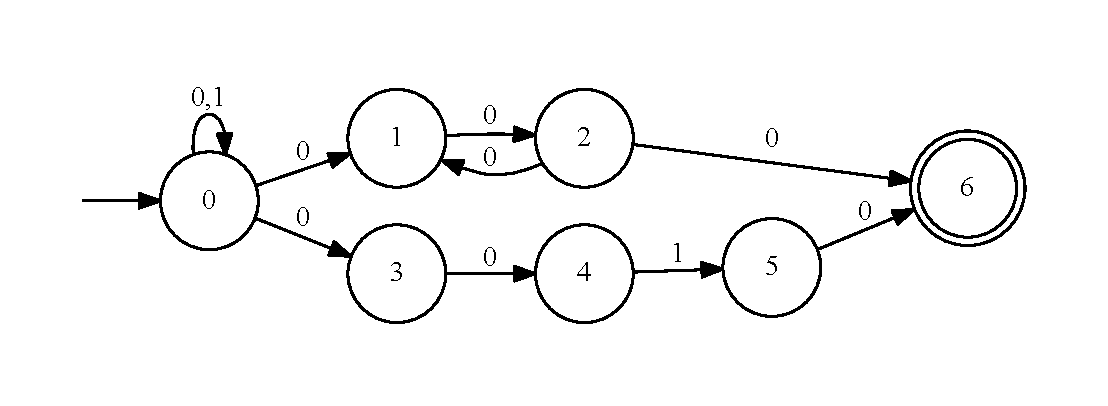
\includegraphics[width=\textwidth]{bilder/nfa_beispiel.pdf}
	\caption{Visuelle Darstellung des NFA zum regulären Ausdruck \texttt{(0|1)*((00)+|001)0}}
	\label{nfa_beispiel}
\end{figure}

\begin{figure}[ht]
	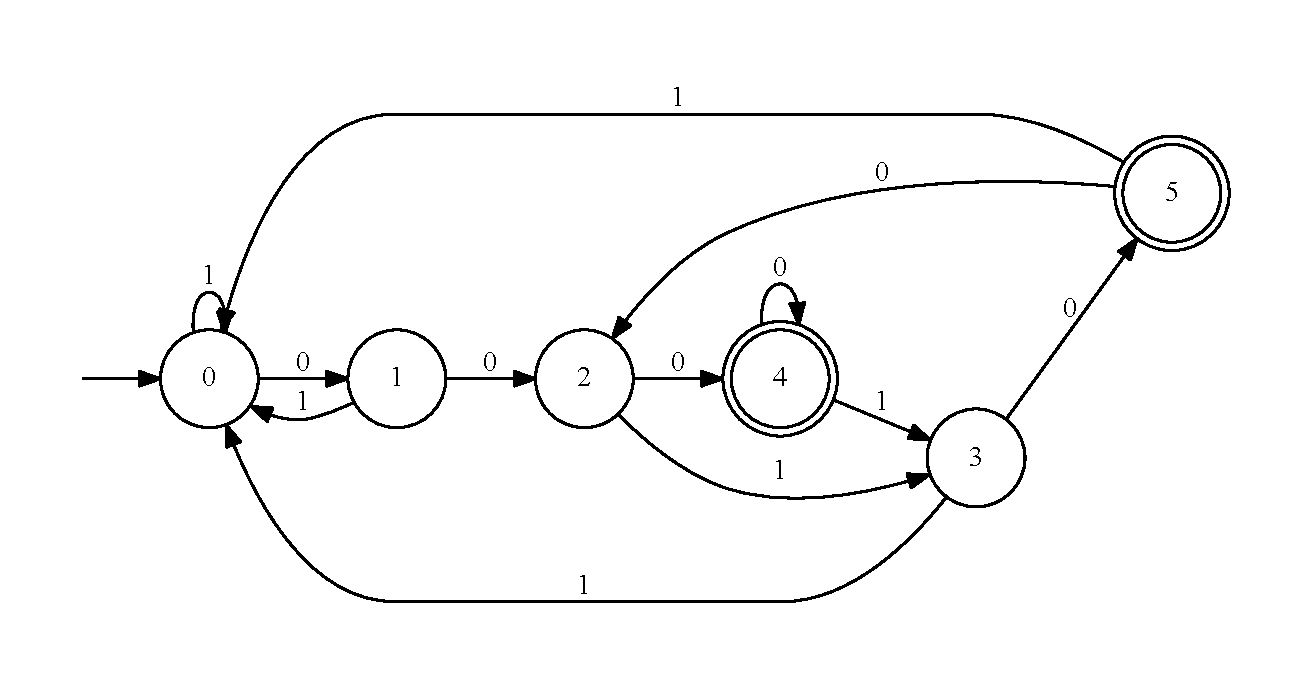
\includegraphics[width=\textwidth]{bilder/dfa_beispiel.pdf}
	\caption{Visuelle Darstellung des DFA zum regulären Ausdruck \texttt{(0|1)*((00)+|001)0}}
	\label{dfa_beispiel}
\end{figure}

\section{Durchführung eines Musterabgleichs}

Der vorgestellte DFA lässt sich als zweidimensionale Übergangstabelle darstellen, die für einen gegebenen Ausgangszustand und ein gelesenes Eingabezeichen den Folgezustand liefert.
Beginnend mit dem Startzustand muss somit lediglich für jedes Zeichen des Eingabewortes der aktuelle Zustand entsprechend der Tabelle angepasst werden und es kann am Ende überprüft werden, ob ein akzeptierender Zustand erreicht wurde.
Dieses Verfahren wird in Abbildung \ref{dfa_matching} schematisch dargestellt.

\begin{figure}[ht]
	\begin{lstlisting}[language=Python]
	dfa = [[1, 0],
		[2, 0],
		[4, 3],
		[5, 0],
		[4, 3],
		[2, 0]]
	cs = 0
	accepting = [4, 5]
	
	word = "010010"
	
	for c in word:
		cs = dfa[cs][int(c)]
	
	if cs in accepting:
		print("Word matches regular expression!")
	\end{lstlisting}
	\caption{Durchführung des Musterabgleichs mithilfe eines DFA}
	\label{dfa_matching}
\end{figure}

\begin{figure}[ht]
	\begin{lstlisting}[language=Python]
	nfa = [[[0, 1, 3], [0]],
		[[2], []],
		[[1, 6], []],
		[[4], []],
		[[], [5]],
		[[6], []],
		[[], []]]
	cs = [0]
	accepting = [6]
	
	word = "010010"
	
	for c in word:
		newCs = []
		for s in cs:
			newCs = newCs + nfa[s][int(c)]
		cs = newCs
	
	for s in cs:
		if s in accepting:
			print("Word matches regular expression!")
			break
	\end{lstlisting}
	\caption{Durchführung des Musterabgleichs mithilfe eines NFA}
	\label{nfa_matching}
\end{figure}

Abbildung \ref{nfa_matching} stellt entsprechend das Verfahren zur Durchführung des Musterabgleichs mittels eines NFAs dar.
Dieses funktioniert sehr ähnlich zu einem DFA, allerdings müssen gegebenenfalls mehrere Zustände gleichzeitig betrachtet werden, wodurch die Auswertung des Automaten komplizierter und zeitaufwändiger wird.

\section{Auswahl eines geeigneten Ansatzes}

Der Nachteil bei der Verwendung von NFAs liegt darin, dass teilweise mehrere Zustände gleichzeitig aktiv sind, da verschiedene Pfade auf einmal verfolgt werden müssen.
Dadurch steigt die Rechenlast beim Lesen von Zeichen und die allgemeine Performanz sinkt.
Bei DFAs ist dies nicht der Fall, da durch den Determinismus zu jeder Zeit klar ist, welche Transition verfolgt werden muss und in welchem Zustand der Automat sich befindet.

Der Nachteil eines DFA liegt allerdings darin, dass dieser im Gegensatz zum NFA eine exponentiell große Anzahl von Zuständen haben kann.
die Zeit für das Verarbeiten eines Strings wird dadurch zwar nicht direkt beeinflusst, allerdings steigt der Speicherverbrauch enorm, wodurch Die Verwendung eines DFA gegebenenfalls unmöglich wird.

Vergangene Arbeiten zeigen, dass ein unkomprimierter DFA die optimale Laufzeit erzielt \cite{Yu2013}.
Außerdem ist nicht zu erwarten, dass im Kontext einer Datenbankanfrage ein hoch komplexer regulärer Ausdruck benötigt wird, sodass der Automat eine effiziente Größe überschreiten würde.
Der exponentiellen Anzahl von Zuständen kann außerdem entgegen gewirkt werden, indem der Automat vor der Verwendung minimiert wird, was in den meisten Anwendungsfällen einen kompakten Automaten ergibt.
Aus diesem Grund wird im folgenden Kapitel ein DFA für den Musterabgleich verwendet.
